\documentclass[12pt]{article}
\usepackage[T1]{fontenc}
\usepackage[utf8]{inputenc}
\usepackage{polski}
\usepackage{minted}
\usepackage{geometry}
\usepackage{natbib}
\usepackage{enumitem}
\usepackage{graphicx}
\usepackage{bold-extra}
\usepackage[font=small,labelfont=bf]{caption}
\usepackage{hyperref}
\usepackage{titlesec}
\hyphenpenalty=10000
\tolerance=1000 \emergencystretch=2em
\titlelabel{\thetitle.\quad}

 \geometry{
     left=23mm,
     top=25mm,
     right=23mm
 }


\def\mydate{\leavevmode\hbox{\twodigits\day.\twodigits\month.\the\year}}
\def\twodigits#1{\ifnum#1<10 0\fi\the#1}

\begin{document}
%titlepage
\thispagestyle{empty}
\begin{center}
\begin{minipage}{0.75\linewidth}
    \centering
    
\includegraphics[width=0.45\linewidth]{agh_logo2.png}
    \par
    \vspace{2cm}
    {\bfseries{\scshape{\Huge  Teoria współbieżności}}}
    \par
    \vspace{2cm}
    {\scshape{\Large Laboratorium 4}}
    \par
    \vspace{0.4cm}
    {\scshape{\Large Java Concurrency Utilities}}
    \par
    \vspace{3cm}

    {\scshape{\Large Albert Gierlach}}\par
    \vspace{1cm}

    {\Large \mydate}
\end{minipage}
\end{center}
\clearpage



\section{Zadanie}
Producenci i konsumenci z losowa ilością pobieranych i wstawianych porcji

\begin{itemize}
    \item Bufor o rozmiarze 2M
    \item Jest m producentów i n konsumentów
    \item Producent wstawia do bufora losowa liczbę elementów (nie więcej niż M)
    \item Konsument pobiera losowa liczbę elementów (nie więcej niż M)
    \item Zaimplementować przy pomocy monitorów Javy oraz mechanizmów Java Concurrency Utilities
    \item Przeprowadzic porownanie wydajnosci vs. rozne parametry, zrobic wykresy i je skomentowac
\end{itemize}

  
\section{Koncept rozwiązania}
Rozwiązanie będzie opierać się na zaimplementowaniu obu metod oraz przeprowadzeniu testów dla różnych konfiguracji. Program w dużej mierze, będzie zależał od losowości, więc dla każdej konfiguracji zostanie przeprowadzone 200 iteracji, a wynikiem będzie średni czas działania programu dla zadanych parametrów. Każdy wątek będzie wykonywał 100 iteracji dodania i pobrania z bufora.

Pierwsza metoda będzie opierać się monitorach. Wątki producentów będą wstrzymywane, gdy w buforze będzie zbyt wiele elementów, a wątki konsumentów gdy będzie zbyt mało. Nad wykonaniem będzie czuwać nadzorca (executor), który zakończy pracę wątków, jeśli jedna ze stron zakończy swoją pracę.

Druga metoda opiera się o gotowe mechanizmy biblioteki Java Concurrent. Wykorzystana zostanie kolejka blokująca (\emph{BlockingQueue}) oraz pula wątków. Podobnie jak w pierwszym wariancie - zostanie wykorzystany nadzorca.

Czasy zostaną zapisane do pliku i na ich podstawie zostaną narysowane wykresy. 

\newpage
\section{Implementacja oraz wyniki}
\begin{minted}[frame=lines,
                framesep=2mm
                ]{java}
public interface IBuffer {
    void unregisterProducer();
    void unregisterConsumer();

    int maxSize();

    void put(int[] products) throws InterruptedException;

    void get(List<Integer> results, int howMany) throws InterruptedException;

    boolean isAnySideInterested();
}

public interface IExecutor {
    void submit(Thread t);

    void shutdownNow();

    void awaitTermination();
}

                
class Producer extends Thread {
    private final IBuffer buffer;
    private final Random random = new Random();
    private final int produceLimit;
    private final int iterations;
    private final IExecutor executor;

    public Producer(IExecutor ex, IBuffer buf, int iters) {
        iterations = iters;
        buffer = buf;
        produceLimit = buffer.maxSize() / 2;
        executor = ex;
    }

    public void run() {
        for(int i = 0; i < iterations; i++) {
            var howMany = Math.max(1, random.nextInt(produceLimit)-1);
            int[] data = new int[howMany];
            IntStream.range(0, howMany).forEach(j -> {
                data[j] = j;
            });

            try {
                buffer.put(data);
            } catch (InterruptedException exception) {
                break;
            }
        }
        buffer.unregisterProducer();
        if(!buffer.isAnySideInterested()){
            executor.shutdownNow();
        }
    }
}

class Consumer extends Thread {
    private final IBuffer buffer;
    private final int consumeLimit;
    private final int iterations;
    private final Random random = new Random();
    private final IExecutor executor;

    public Consumer(IExecutor ex, IBuffer buf, int iters) {
        iterations = iters;
        buffer = buf;
        consumeLimit = buffer.maxSize() / 2;
        executor = ex;
    }

    public void run() {
        for (int i = 0; i < iterations; i++) {
            var howMany = Math.max(1, random.nextInt(consumeLimit)-1);
            List<Integer> results = new LinkedList<>();
            try {
                buffer.get(results, howMany);
            } catch (InterruptedException exception) {
                break;
            }
        }

        buffer.unregisterConsumer();
        if (!buffer.isAnySideInterested()) {
            executor.shutdownNow();
        }
    }
}

public class MyExecutor implements IExecutor {
    private final List<Thread> workers = new LinkedList<>();

    @Override
    public void submit(Thread t){
        workers.add(t);
    }

    @Override
    public void shutdownNow(){
        workers.forEach(Thread::interrupt);
    }

    @Override
    public void awaitTermination() {
        workers.forEach(Thread::start);

        workers.forEach(t -> {
            try {
                t.join();
            } catch (InterruptedException ignored) {
            }
        });
    }
}

public class ExecutorServiceWrapper implements IExecutor {
    private final ExecutorService executorService;
    private final List<Thread> workers = new LinkedList<>();

    public ExecutorServiceWrapper(int threadNum) {
        executorService = Executors.newFixedThreadPool(threadNum);
    }

    @Override
    public void submit(Thread t) {
        workers.add(t);
    }

    @Override
    public void shutdownNow() {
        executorService.shutdownNow();
    }

    @Override
    public void awaitTermination() {
        workers.forEach(executorService::submit);

        executorService.shutdown();
        try {
            executorService.awaitTermination(Long.MAX_VALUE, TimeUnit.NANOSECONDS);
        } catch (InterruptedException ignored) {
        }
    }
}

class Buffer implements IBuffer {
    private final LinkedList<Integer> buffer = new LinkedList<>();
    private final int maxBufferSize;
    private final Object lock = new Object();
    private Integer producersRunning;
    private Integer consumersRunning;

    public Buffer(int size, int m, int n) {
        maxBufferSize = size * 2;
        producersRunning = m;
        consumersRunning = n;
    }

    @Override
    public void unregisterProducer() {
        synchronized (lock) {
            producersRunning--;
        }
    }

    @Override
    public void unregisterConsumer() {
        synchronized (lock) {
            consumersRunning--;
        }
    }

    @Override
    public boolean isAnySideInterested() {
        return producersRunning > 0 && consumersRunning > 0;
    }

    @Override
    public int maxSize() {
        return maxBufferSize;
    }

    @Override
    public synchronized void put(int[] products) throws InterruptedException {
        while (isAnySideInterested() && 
                (buffer.size() + products.length >= maxBufferSize)) {
            wait();
        }

        if (!isAnySideInterested()) {
            return;
        }

        buffer.addAll(Arrays.stream(products).boxed().collect(Collectors.toList()));
        notifyAll();
    }

    @Override
    public synchronized void get(List<Integer> results, 
                                    int howMany) throws InterruptedException {
        while (isAnySideInterested() && buffer.size() < howMany) {
            wait();
        }

        if (!isAnySideInterested()) {
            return;
        }

        var sublist = buffer.subList(0, howMany);
        for(int i = 0; i < howMany; i++){
            var v = sublist.get(i);
            results.add(v);
        }
        sublist.clear();
        notifyAll();
    }
}

class Buffer2 implements IBuffer {
    private final int maxBufferSize;
    private final AtomicInteger producersRunning;
    private final AtomicInteger consumersRunning;
    private final BlockingQueue<Integer> buffer;

    public Buffer2(int size, int m, int n) {
        maxBufferSize = size * 2;
        producersRunning = new AtomicInteger(m);
        consumersRunning = new AtomicInteger(n);
        buffer = new ArrayBlockingQueue<>(maxBufferSize);
    }

    @Override
    public void unregisterProducer() {
        producersRunning.decrementAndGet();
    }

    @Override
    public void unregisterConsumer() {
        consumersRunning.decrementAndGet();
    }

    @Override
    public boolean isAnySideInterested() {
        return producersRunning.get() > 0 && consumersRunning.get() > 0;
    }

    @Override
    public int maxSize() {
        return maxBufferSize;
    }

    @Override
    public void put(int[] products) throws InterruptedException {
        for (var v : products) {
            if(!isAnySideInterested()){
                return;
            }
            buffer.put(v);
        }
    }

    @Override
    public void get(List<Integer> results, int howMany) throws InterruptedException {

        while (results.size() < howMany) {
            if(!isAnySideInterested()){
                return;
            }
            Integer v = buffer.take();
            results.add(v);
        }
    }
}

public class PKMain {
    enum MODE {
        MODE_MONITORS,
        MODE_CONCURRENT_LIB
    }

    public static void main(String[] args) {
        var producers = List.of(3, 10, 20);
        var consumers = List.of(3, 10, 20);
        var bufferSizes = List.of(5, 10, 50, 100);

        var results = new LinkedList<String>();

        for (var p : producers) {
            for (var c : consumers) {
                for (var bs : bufferSizes) {
                    var avg1 = testCaseWrapper(p, c, bs, MODE.MODE_MONITORS);
                    var avg2 = testCaseWrapper(p, c, bs, MODE.MODE_CONCURRENT_LIB);


                    results.add(p + ", " + c + ", " + 
                            bs + ", " + round(avg1, 2) + ", " + round(avg2, 2));
                }
            }
        }

        Path out = Paths.get("results.csv");
        try {
            Files.write(out, results, Charset.defaultCharset());
        } catch (IOException e) {
            e.printStackTrace();
        }
    }

    public static double round(double v, int places){
        v = Math.round(v * Math.pow(10, places));
        v = v / Math.pow(10, places);
        return v;
    }

    public static double testCaseWrapper(int prodNum, int consNum, 
                int halfBufSize, MODE mode) {
        var times = new LinkedList<Long>();

        IntStream.range(0, 200).forEach(i -> {
            long before = System.currentTimeMillis();

            if (mode == MODE.MODE_CONCURRENT_LIB) {
                testConcurrentLibrary(prodNum, consNum, halfBufSize);
            } else {
                testMonitors(prodNum, consNum, halfBufSize);
            }

            long after = System.currentTimeMillis();
            long diff = after - before;
            times.add(diff);
        });

        return times.stream().mapToLong(i -> i).average().getAsDouble();
    }

    public static void testConcurrentLibrary(int m, int n, int M) {
        var buffer = new Buffer2(M, m, n);
        var executor = new ExecutorServiceWrapper(n+m);

        runTasks(m, n, buffer, executor);
    }

    public static void testMonitors(int m, int n, int M) {
        var buffer = new Buffer(M, m, n);
        var executor = new MyExecutor();

        runTasks(m, n, buffer, executor);
    }

    public static void runTasks(int m, int n, IBuffer buffer, IExecutor executor){
        IntStream.range(0, n).forEach(i ->
                executor.submit(
                        new Consumer(executor, buffer, 100)
                ));
        IntStream.range(0, m).forEach(i ->
                executor.submit(
                        new Producer(executor, buffer, 100)
                ));

        executor.awaitTermination();
    }
}

\end{minted}

\noindent
Po wykonaniu programu został stworzony plik results.csv. Wyniki prezentują się następująco:
\begin{center}
\centering
    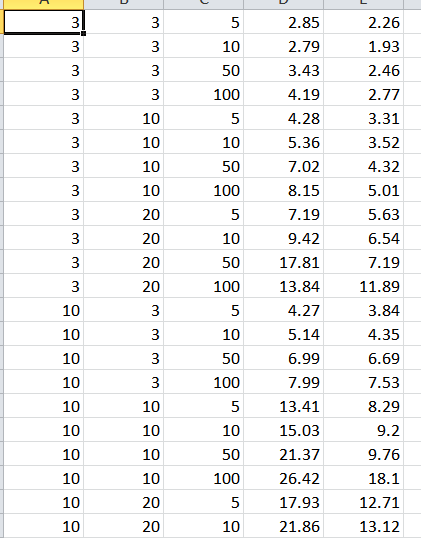
\includegraphics[scale=0.8]{csv.png}
\end{center}
\newpage


\section{Wnioski}
Na podstawie danych zostały wygenerowane wykresy przedstawiające czasy działania programu dla konkretnych konfiguracji. Tytuł wykresów mówi o liczbie producentów i konsumentów.

\begin{center}
\centering
    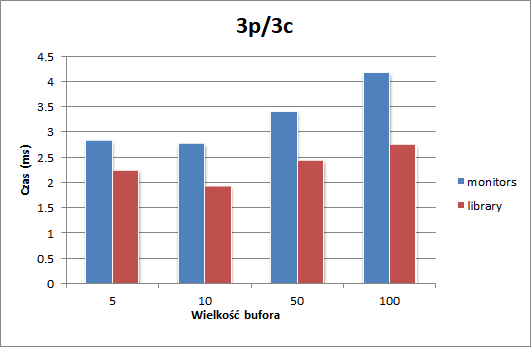
\includegraphics[width=\textwidth]{1.png}
    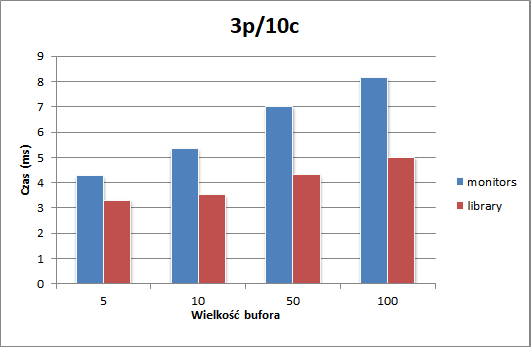
\includegraphics[width=\textwidth]{2.png}
    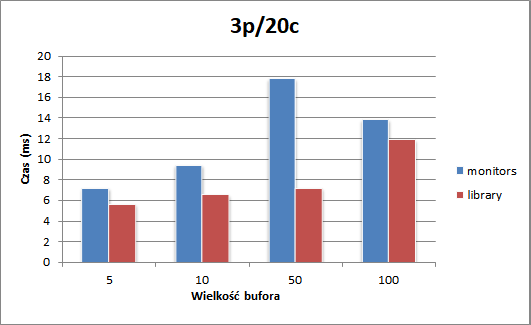
\includegraphics[width=\textwidth]{3.png}
    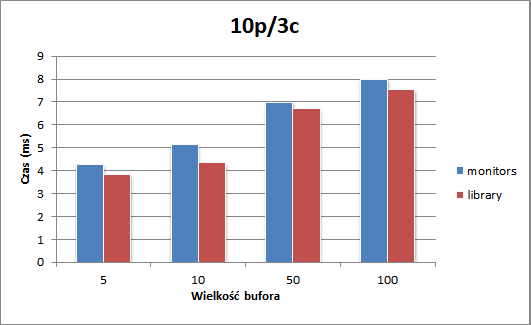
\includegraphics[width=\textwidth]{4.png}
    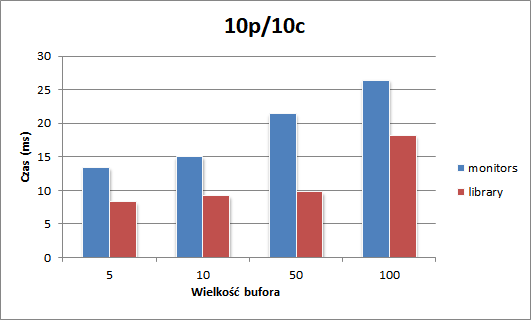
\includegraphics[width=\textwidth]{5.png}
    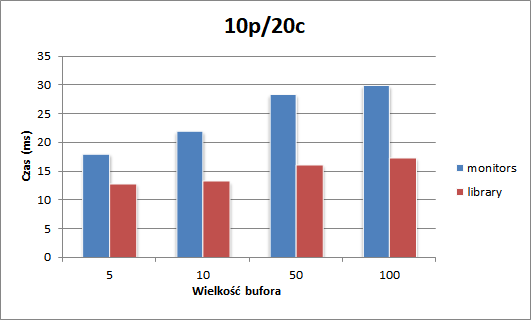
\includegraphics[width=\textwidth]{6.png}
    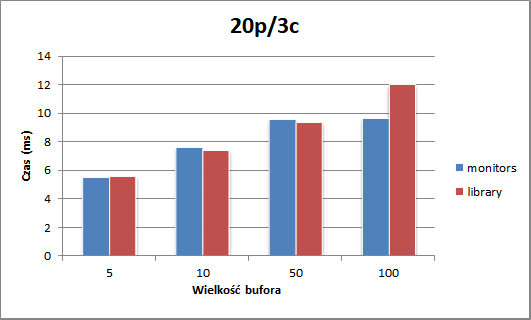
\includegraphics[width=\textwidth]{7.png}
    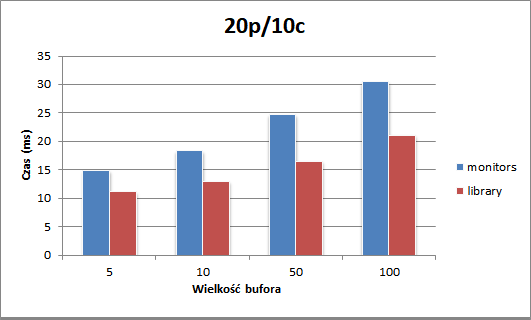
\includegraphics[width=\textwidth]{8.png}
    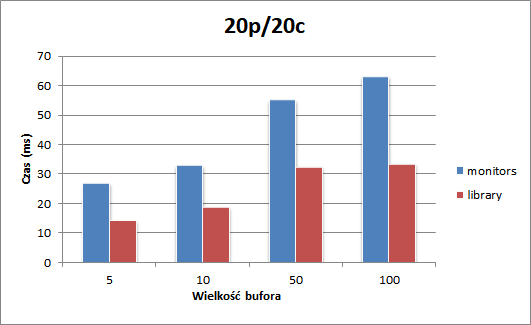
\includegraphics[width=\textwidth]{9.png}
    
\end{center}

\newpage
Na podstawie powyższych wykresów, można zauważyć, że w niemalże każdym przypadku, wersja problemu producentów-konsumentów zaimplementowana za pomocą monitorów jest wolniejsza od rozwiązania za pomocą Java Concurrent Library. Największe różnice w czasach widać, gdy liczba konsumentów jest większa niż liczba producentów.
W przypadku gdy liczba producentów była znacznie większa niż liczba konsumentów wyniki są bardzo do siebie zbliżone. 
\\

Warto dodać, że biblioteka Java Concurrent umożliwia korzystanie z kontenerów, które mają synchronizowany dostęp (np. \emph{BlockingQueue}), mechanizmów synchronizacji jak: \emph{Sempahore}, \emph{CyclicBarrier}, \emph{CountdownLatch}, \emph{Lock}, \emph{Condition} oraz zmiennych atomowych (np. \emph{AtomicInteger}). Używanie gotowych rozwiązań ogranicza także możliwość pomyłki podczas implementacji.




\end{document}
